\textbf{Входные параметры:}
 
 VectorOfProbability --- массив вероятностей выбора индивидов для ранговой селекции;
 
 VMHL\_N --- размер массива VectorProbability.

\textbf{Возвращаемое значение:} 

 Номер выбранного индивида популяции.

 \textbf{Принцип работы:}

\begin{figure} [h]
  \center
  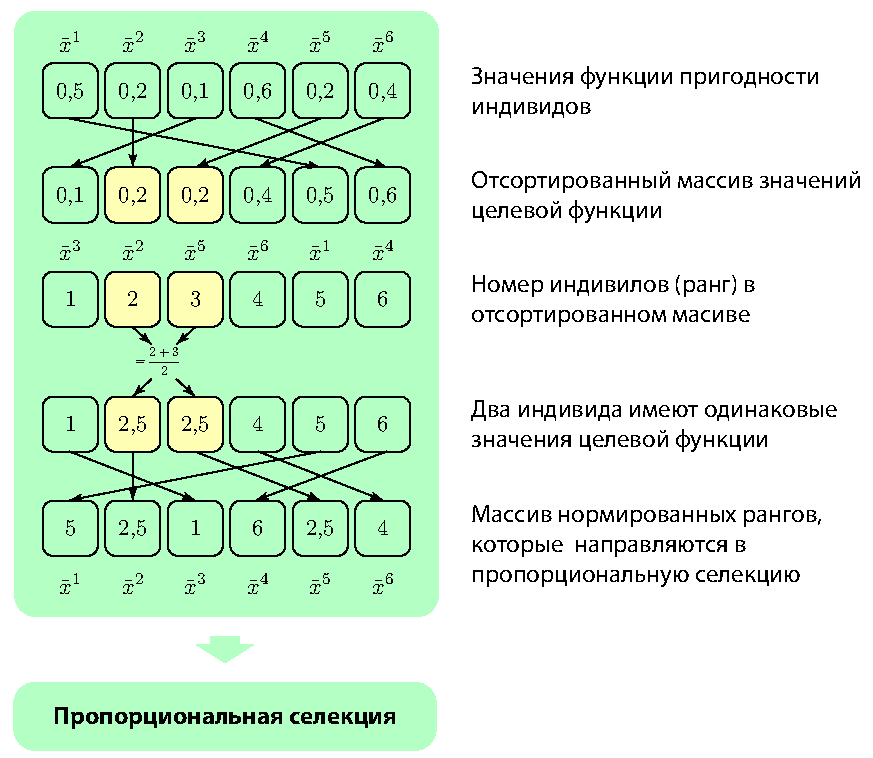
\includegraphics [scale=0.8] {MHL_RankSelection_Sheme}
  \caption{Механизм работы ранговой селекции} 
  \label{img:MHL_RankSelection_Sheme}  
\end{figure}

\textbf{О функции:}

Данная функция используется в стандартном генетическом алгоритме, реализованным в виде функции MHL\_StandartGeneticAlgorithm. Работает в связке с функциями MHL\_MakeVectorOfRankForRankSelection и MHL\_MakeVectorOfProbabilityForProportionalSelectionV2. Оператор селекции работает с массивом пригодностей индивидов, но непосредственно ранговая селекция выбирает индивида исходя из рангов индивидов, преобразованных в вероятности выбора. Каждый раз для выбора индивида создавать массив вероятностей и рангов затратно, поэтому для каждой популяции на каждом поколении вначале вызывается функция MHL\_MakeVectorOfRankForRankSelection для генерации вектора рангов, а затем MHL\_MakeVectorOfProbabilityForProportionalSelectionV2 для генерации вектора вероятностей выбора индивида, а затем этот массив и подставляется в ранговую селекцию.
  
\textbf{Примечание:}

На рисунке показано, что ранги подаются в пропорциональную селекцию, но из кода этого не видно. Но по своей сути код данной функции повторяет код функции MHL\_ProportionalSelectionV2 и также требует вектор вероятностей выбора. Так что всё соответствует рисунку.

